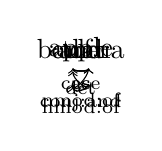
\begin{tikzpicture}
[
every edge/.style={in=270, out=270, draw=black!250}
]
\tikzset{frontier/.style={distance from root=170pt}}
\Tree [.ROOT [.NP [.NP [.DT \node (the) {the}; ]
                       [.NN \node (color) {color}; ]
                  ]
                  [.PP [.IN \node (of) {of}; ]
                       [.NP [.NP [.NN \node (banana) {banana}; ] ]
                            [.CC \node (and) {and}; ]
                            [.NN \node (apple) {apple}; ]
                       ]
                  ]
             ]
      ]

\path[->]
([xshift=-1mm, yshift=0mm] color.south)	edge[looseness=0.50] node[below] {\scriptsize det}	([xshift=1mm, yshift=0mm] the.south)
([xshift=-1mm, yshift=0mm] banana.south)	edge[looseness=0.50] node[below] {\scriptsize case}	([xshift=1mm, yshift=0mm] of.south)
([xshift=1mm, yshift=0mm] banana.south)	edge[looseness=0.50] node[below] {\scriptsize cc}	([xshift=-1mm, yshift=0mm] and.south)
([xshift=1mm, yshift=0mm] color.south)	edge[looseness=1.00] node[below] {\scriptsize nmod:of}	([xshift=-1mm, yshift=-2mm] banana.south)
([xshift=1mm, yshift=-2mm] banana.south)	edge[looseness=1.00] node[below] {\scriptsize conj:and}	([xshift=-1mm, yshift=0mm] apple.south)
([xshift=1mm, yshift=-2mm] color.south)	edge[looseness=1.00] node[below] {\scriptsize nmod:of}	([xshift=-1mm, yshift=-2mm] apple.south);
\end{tikzpicture}
